\documentclass[tikz,border=2pt]{standalone}
\usepackage{times}
\usepackage{amsmath,amssymb}
\usetikzlibrary{arrows.meta,calc,positioning,fit,backgrounds}
\definecolor{ink}{HTML}{0b0b0b}
\definecolor{sub}{HTML}{52514e}
\definecolor{axis}{HTML}{9a9994}
\definecolor{ours}{HTML}{2a78d6}
\definecolor{tint}{HTML}{eef4fc}
\definecolor{warm}{HTML}{eb6834}
\definecolor{warmtint}{HTML}{fdf0ea}
\definecolor{greytint}{HTML}{f3f3f1}
\begin{document}
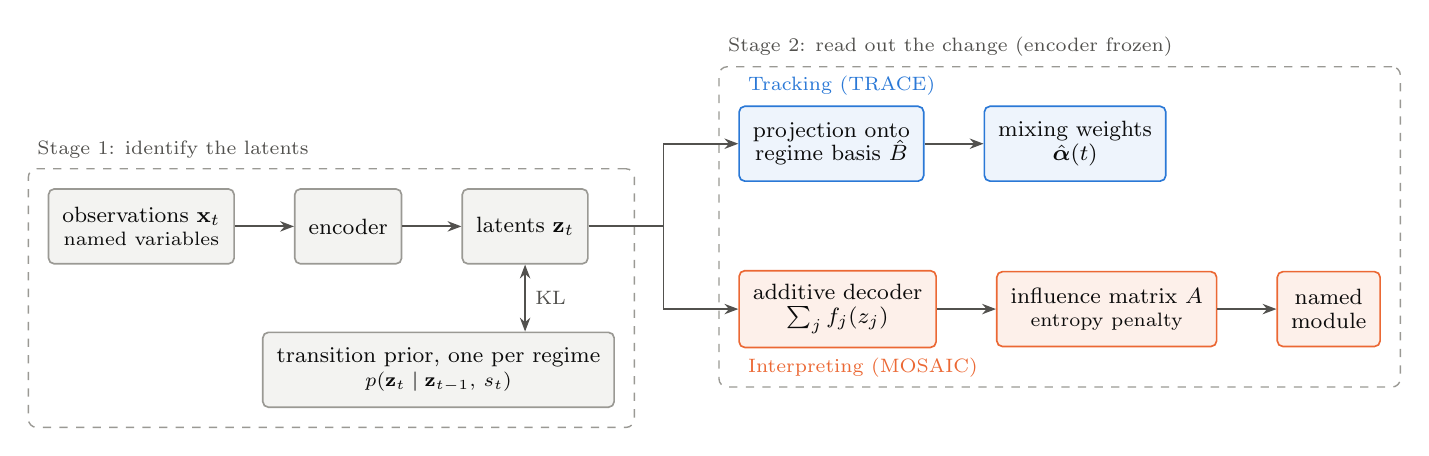
\begin{tikzpicture}[font=\footnotesize, text=ink, >={Stealth[length=5pt]},
    box/.style={draw=axis, line width=0.6pt, rounded corners=2pt, fill=greytint, align=center, inner sep=5pt, minimum height=0.95cm},
    tr/.style={box, draw=ours, fill=tint},
    mo/.style={box, draw=warm, fill=warmtint},
    lab/.style={font=\scriptsize, text=sub, align=center},
    arr/.style={->, line width=0.7pt, draw=sub}]

  % ---------------- Stage 1
  \node[box] (x) {observations $\mathbf{x}_t$\\[-1pt]{\scriptsize named variables}};
  \node[box, right=0.75cm of x] (enc) {encoder};
  \node[box, right=0.75cm of enc] (z) {latents $\mathbf{z}_t$};
  \node[box, below=0.85cm of z, xshift=-1.1cm] (prior) {transition prior, one per regime\\[-1pt]{\scriptsize $p(\mathbf{z}_t\mid\mathbf{z}_{t-1},\,s_t)$}};
  \draw[arr] (x) -- (enc);
  \draw[arr] (enc) -- (z);
  \draw[<->, line width=0.7pt, draw=sub] (z.south) -- node[lab, right] {KL} (z.south |- prior.north);

  % ---------------- Stage 2, tracking
  \node[tr, right=1.9cm of z, yshift=1.05cm] (proj) {projection onto\\[-1pt]regime basis $\hat B$};
  \node[tr, right=0.75cm of proj] (alpha) {mixing weights\\[-1pt]$\hat{\boldsymbol{\alpha}}(t)$};
  \draw[arr] (z.east) -- ++(0.95,0) |- (proj.west);
  \draw[arr] (proj) -- (alpha);

  % ---------------- Stage 2, interpreting
  \node[mo, right=1.9cm of z, yshift=-1.05cm] (dec) {additive decoder\\[-1pt]$\sum_j f_j(z_j)$};
  \node[mo, right=0.75cm of dec] (A) {influence matrix $A$\\[-1pt]{\scriptsize entropy penalty}};
  \node[mo, right=0.75cm of A] (mod) {named\\[-1pt]module};
  \draw[arr] (z.east) -- ++(0.95,0) |- (dec.west);
  \draw[arr] (dec) -- (A);
  \draw[arr] (A) -- (mod);

  \node[lab, text=ours, anchor=south west] at (proj.north west) {Tracking (TRACE)};
  \node[lab, text=warm, anchor=north west] at (dec.south west) {Interpreting (MOSAIC)};

  % ---------------- stage frames
  \begin{scope}[on background layer]
    \node[draw=axis, dashed, line width=0.5pt, rounded corners=3pt, inner sep=7pt, fit=(x)(enc)(z)(prior)] (s1) {};
    \node[draw=axis, dashed, line width=0.5pt, rounded corners=3pt, inner xsep=7pt, inner ysep=14pt, fit=(proj)(alpha)(dec)(A)(mod)] (s2) {};
  \end{scope}
  \node[lab, anchor=south west] at (s1.north west) {Stage 1: identify the latents};
  \node[lab, anchor=south west] at (s2.north west) {Stage 2: read out the change (encoder frozen)};
\end{tikzpicture}
\end{document}
